\chapter{Stato dell'arte}
\label{chap:stateofart}
Illustriamo ora lo stato dell'arte delle varie tecniche e tecnologie che coinvolgono il bot.
\section{Machine Learning}
Il machine learning (in seguito, ML) è una disciplina che si occupa di rispondere, sostanzialmente, a due domande: \textit{Come si può costruire un sistema informatico che migliora con l'esperienza?} e \textit{Quali sono le leggi teoriche fondamentali che governano ogni sistema di apprendimento, sia esso implementato nei computer, negli umani, nelle organizzazioni?}. Il ML copre una serie di compiti diversi, dalla classificazione di email spam, al riconoscimento facciale, al controllo di robot \cite{book:mitchell1997machine}. Ogni problema di ML può essere riassunto come il miglioramento di una determinata performance (data, ad esempio, dall'errore sulle predizioni di un algoritmo di classificazione) durante l'esecuzione di un'operazione. Seguendo l'esempio delle email spam, un algoritmo di ML potrebbe apprendere, tramite un \textit{training set} di email già etichettate come spam/non-spam, a categorizzarne altre.
Portando il problema in termini matematici, vogliamo, dato il grafico della figura \ref{fig:noncategorized-spam},
\begin{figure}[H]
  \begin{center}
    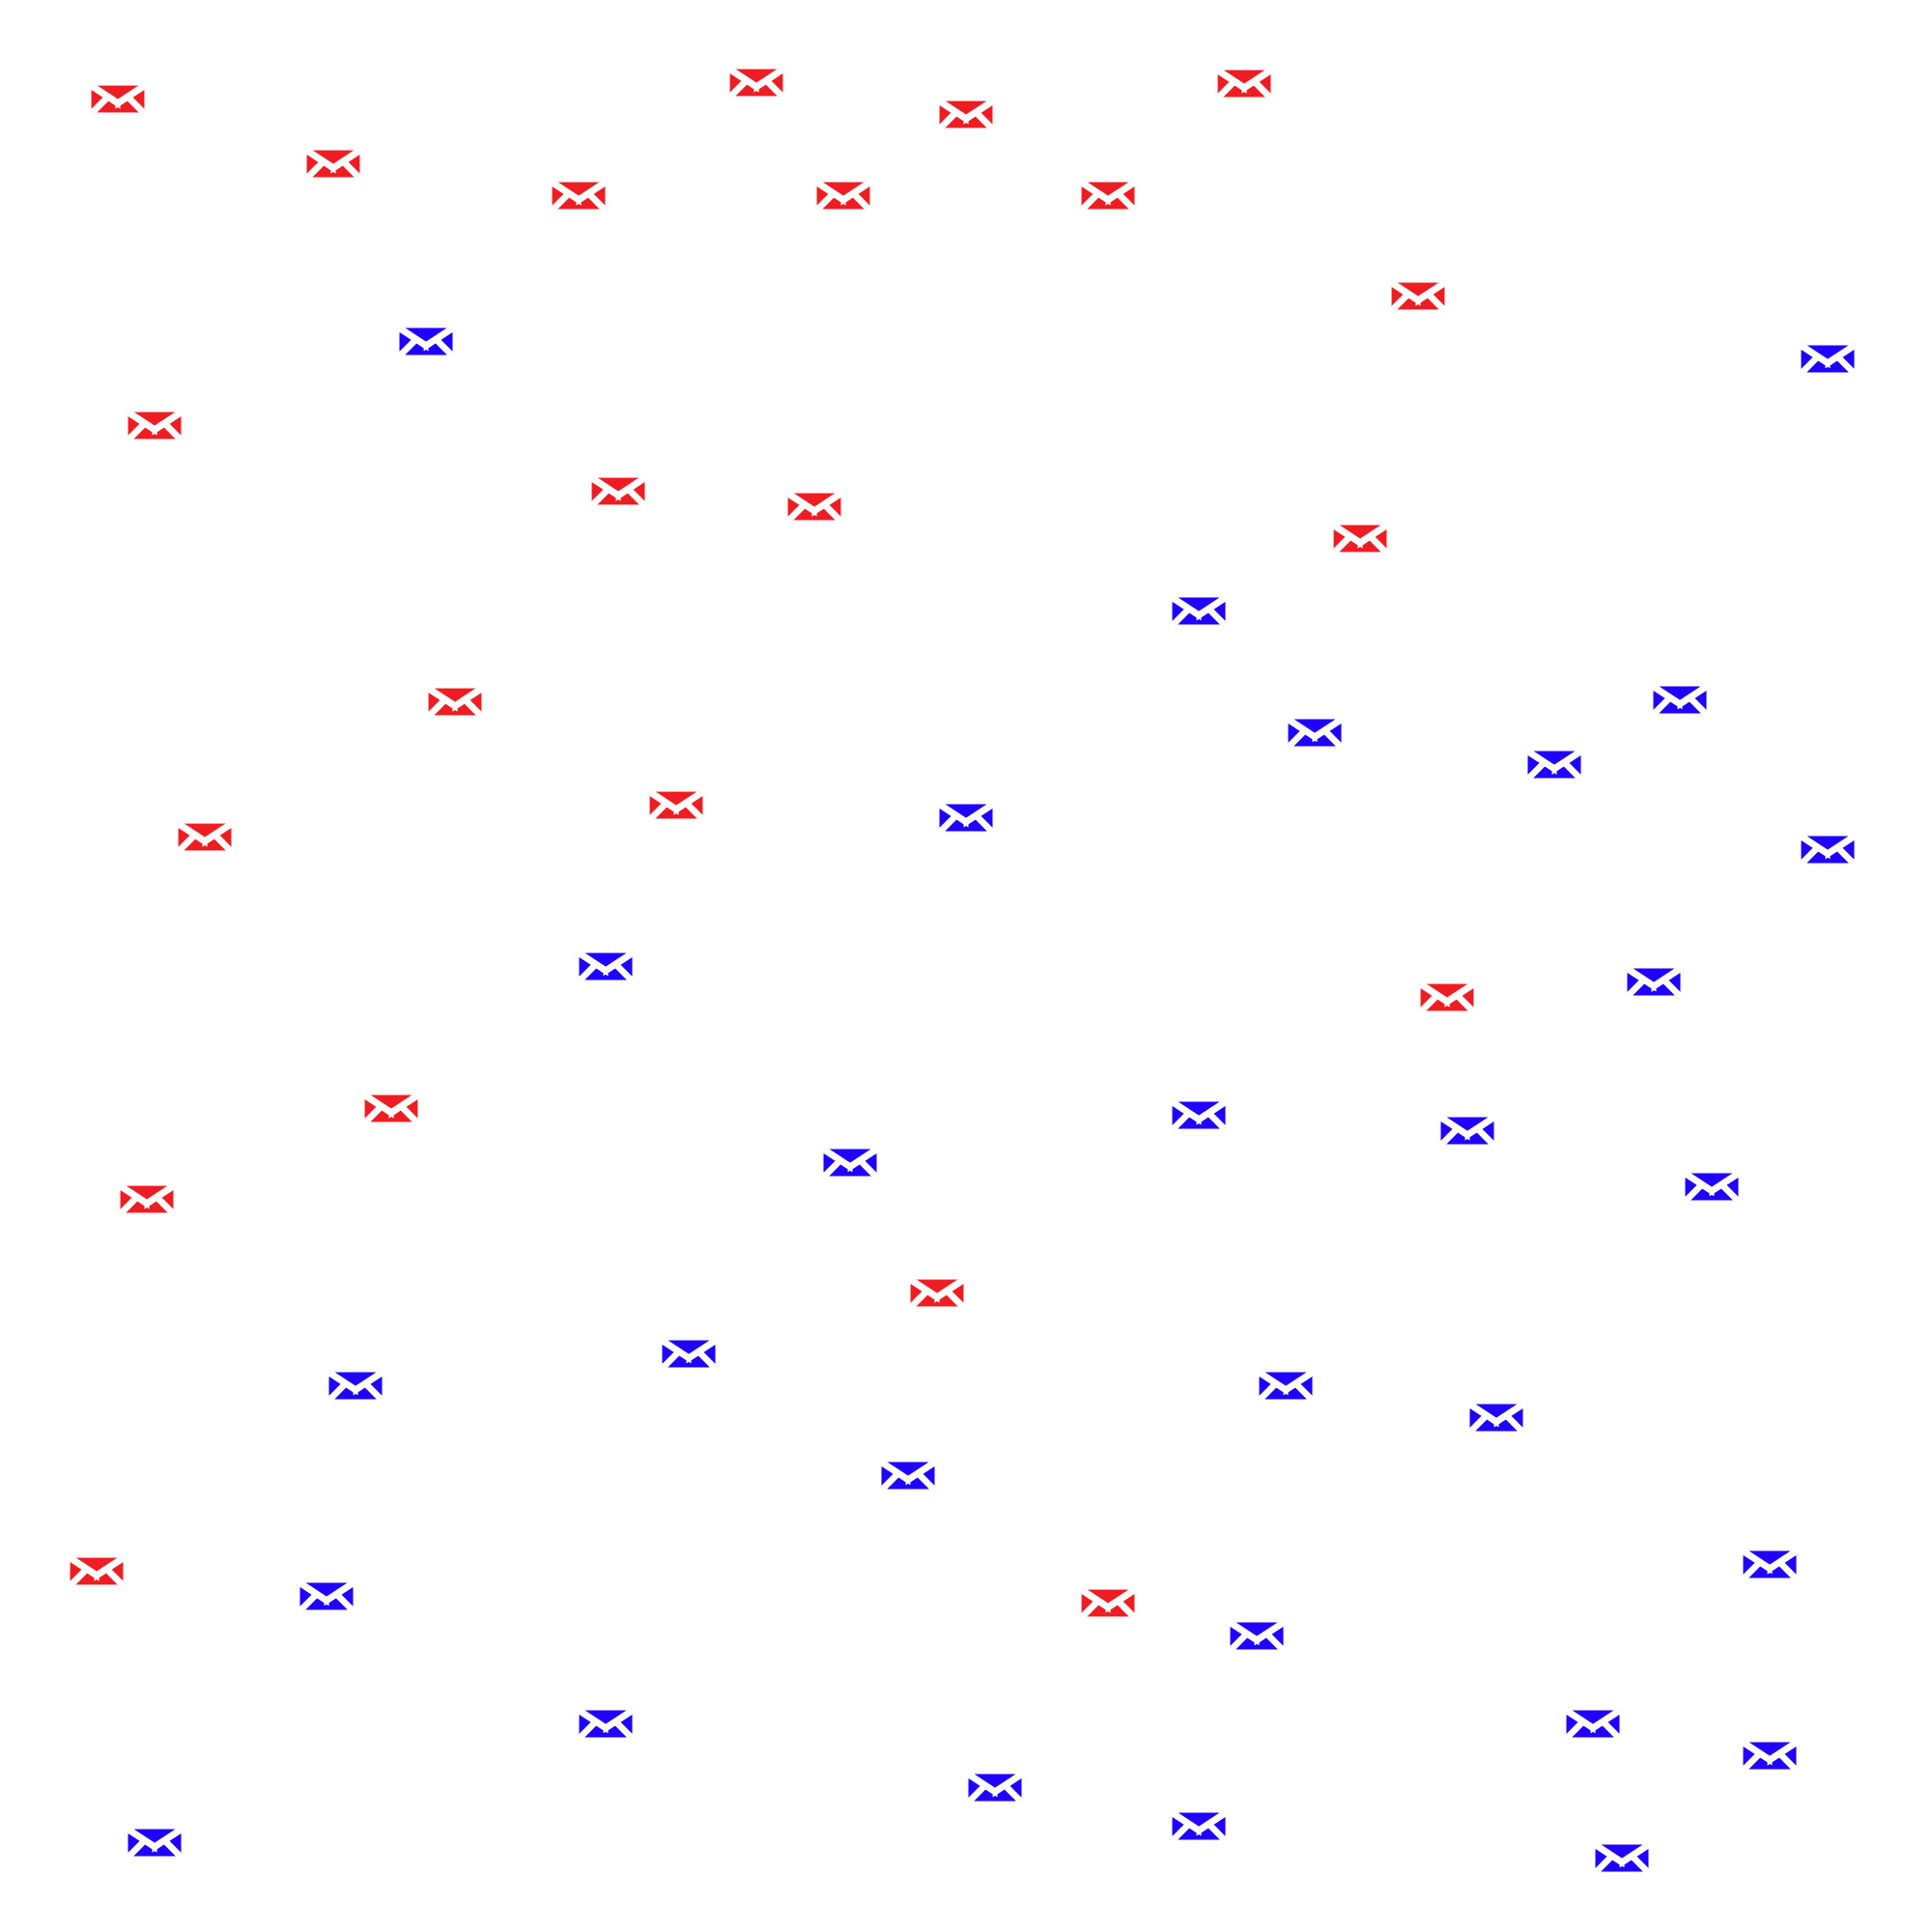
\includegraphics[width=0.8\columnwidth]{images/stateofart/noncategorized-spam.jpg}
  \end{center}
  \caption{Email spam/non-spam}
  \label{fig:noncategorized-spam}
\end{figure}
in cui i simboli rossi sono email spam, e quelli blu no, trovare una funzione che ci permetta di evidenziare le email da eliminare. Ciò che faremo sarà quindi definire un insieme di \textbf{features}, consistenti, ad esempio, nel contenuto testuale della mail (vettorizzato in termini numerici), l'orario di arrivo, la lunghezza in parole, etc\dots Oltre a ciò, definiremo una \textbf{label}, ossia la caratteristica che vogliamo predire: sarà, per esempio, 1 se l'email è spam, 0 altrimenti. Ora, il problema consiste in una semplice regressione lineare: date le features $x_0, x_1, x_2$ e la label $y$, vogliamo trovare dei pesi $w_0, w_1, w_2$ tali che
\begin{displaymath}
  w_0x_0+w_1x_1+w_2x_2
\end{displaymath}
approssimi al meglio $y$. Per fare ciò, procediamo per iterazioni: partiremo con dei pesi arbitrari, calcolando $y$ per ogni esempio (già etichettato) fornito, e ne calcoleremo l'errore rispetto alla $y$ reale. Potremo quindi calcolare il gradiente (ossia la somma delle derivate parziali sui rispettivi pesi) della funzione che lega l'errore ai pesi $w_i$, ottenendone un'informazione fondamentale: indicherà infatti \textbf{la direzione nella quale la funzione errore è decrescente}. Ci potremo quindi spostare, di una quantità pari al \textit{learning rate} (uno degli iperparametri definiti arbitrariamente), nella direzione di diminuzione dell'errore. Scegliere un corretto \textit{learning rate} è una parte fondamentale dello sviluppo dell'algoritmo di ML: se è troppo piccolo, la soluzione richiederà troppo tempo, se troppo grande, la soluzione non sarà abbastanza precisa. Dopo un sufficiente numero di esecuzioni dell'algoritmo, il nostro grafico avrà ora l'aspetto in figura \ref{fig:categorized-spam}.
\begin{figure}[H]
  \begin{center}
    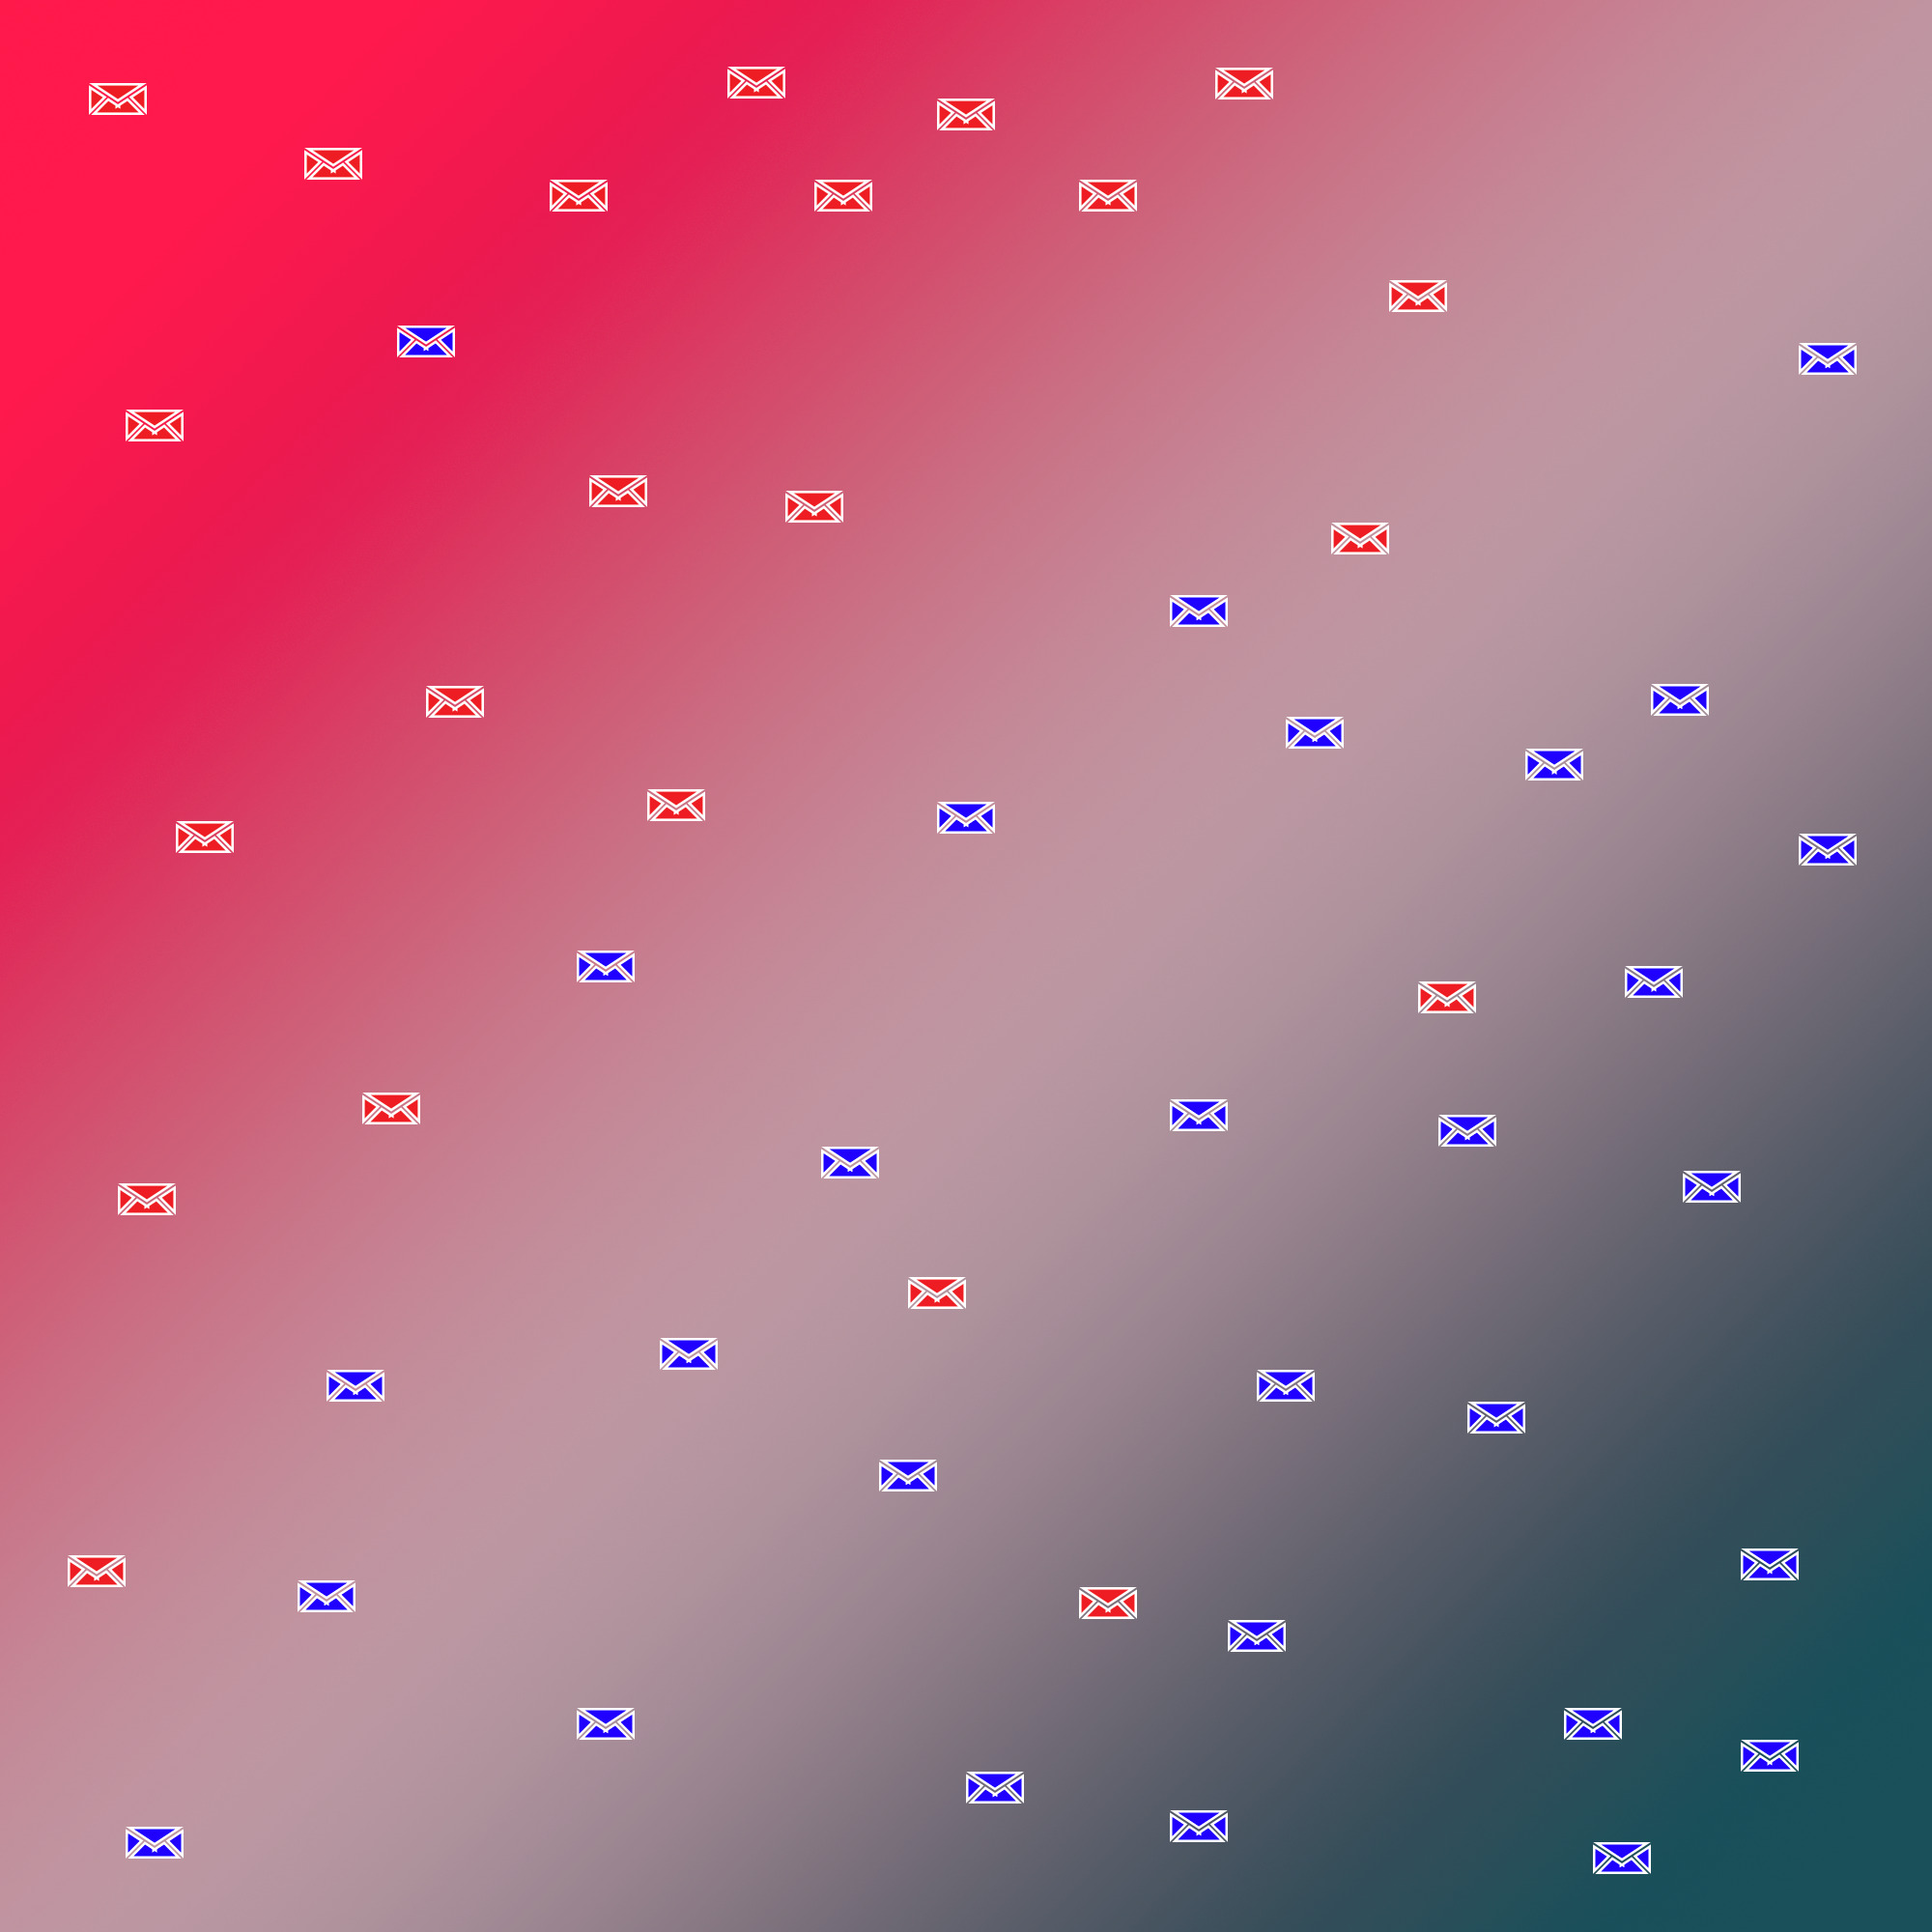
\includegraphics[width=0.8\columnwidth]{images/stateofart/categorized-spam.jpg}
  \end{center}
  \caption{Categorizzazione del dataset}
  \label{fig:categorized-spam}
\end{figure}
Saremo quindi in grado di determinare, con una determinata \textit{accuracy} (in questo caso data dall'opacità del colore di sfondo), l'appartenenza di un esempio ad una classe o all'altra.
\subsection{Reti neurali}
Per illustrare il concetto di rete neurale, produciamo anzitutto un grafico del modello lineare appena definito \ref{fig:linear-NN}.
\begin{figure}[H]
  \begin{center}
    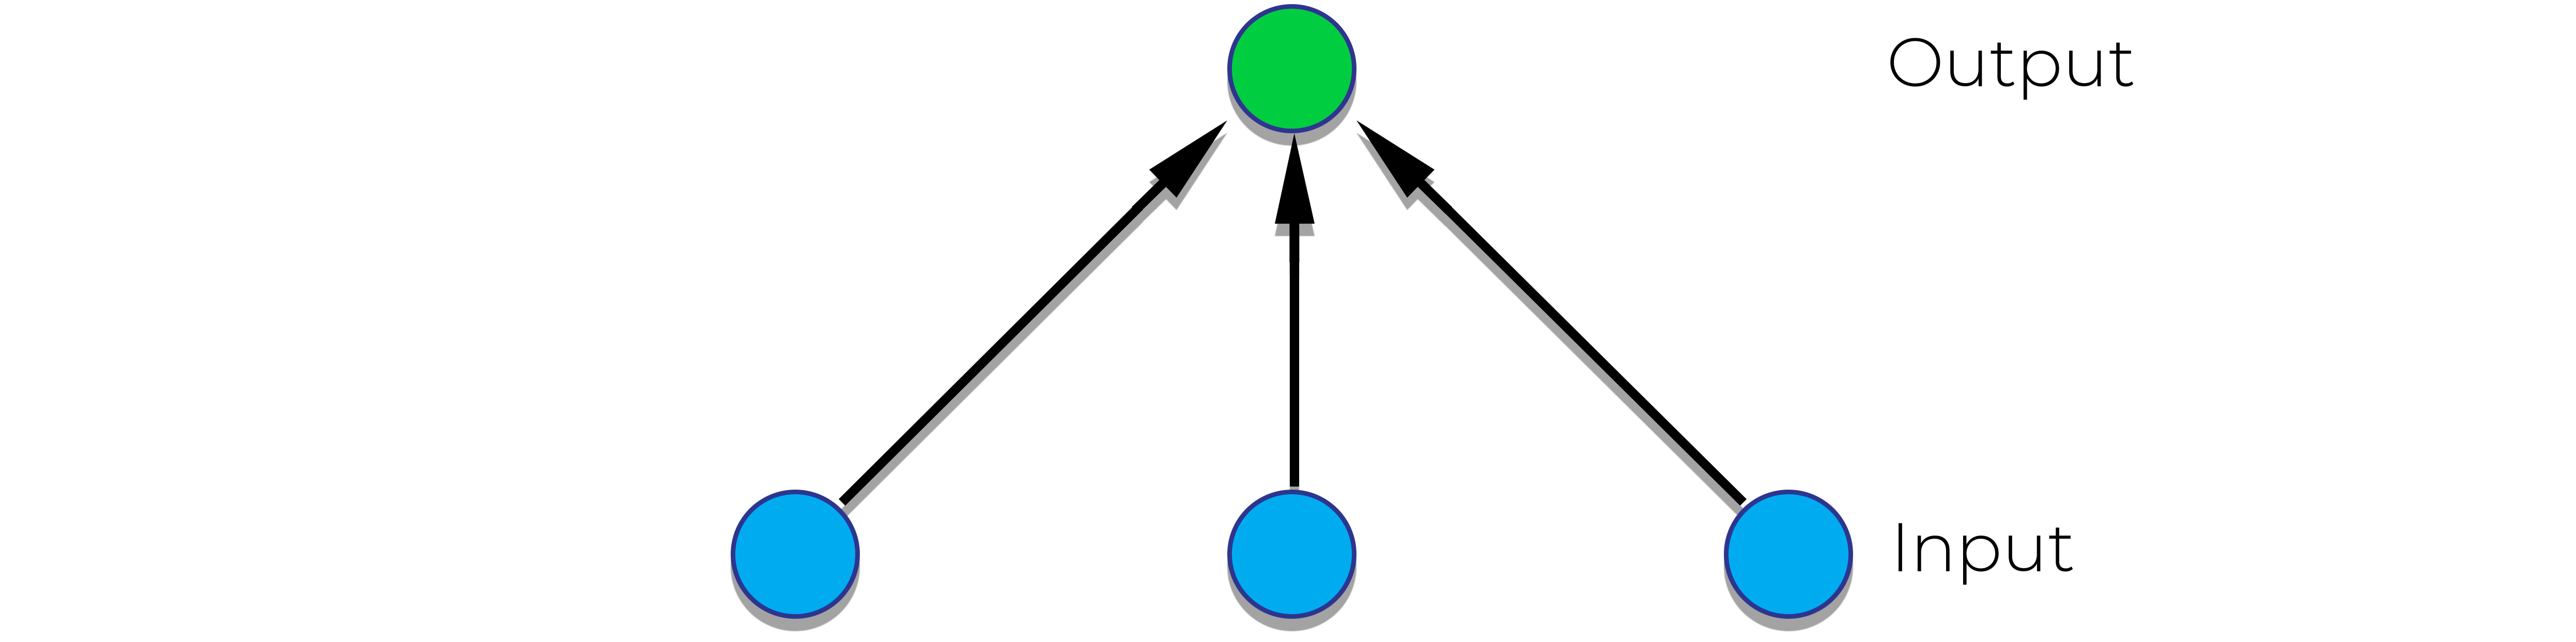
\includegraphics[width=0.8\columnwidth]{images/stateofart/linear-NN.jpg}
  \end{center}
  \caption{Modello lineare}
  \label{fig:linear-NN}
\end{figure}
Ogni cerchio blu rappresenta una feature, ed il cerchio verde rappresenta la somma pesata degli input. Vorremmo che questo modello fosse in grado di approssimare anche problemi non-lineari. Potremmo quindi decidere di inserire un nuovo strato di valori intermedi, ottenendo il modello in figura \ref{fig:double-linear-NN}:
\begin{figure}[H]
  \begin{center}
    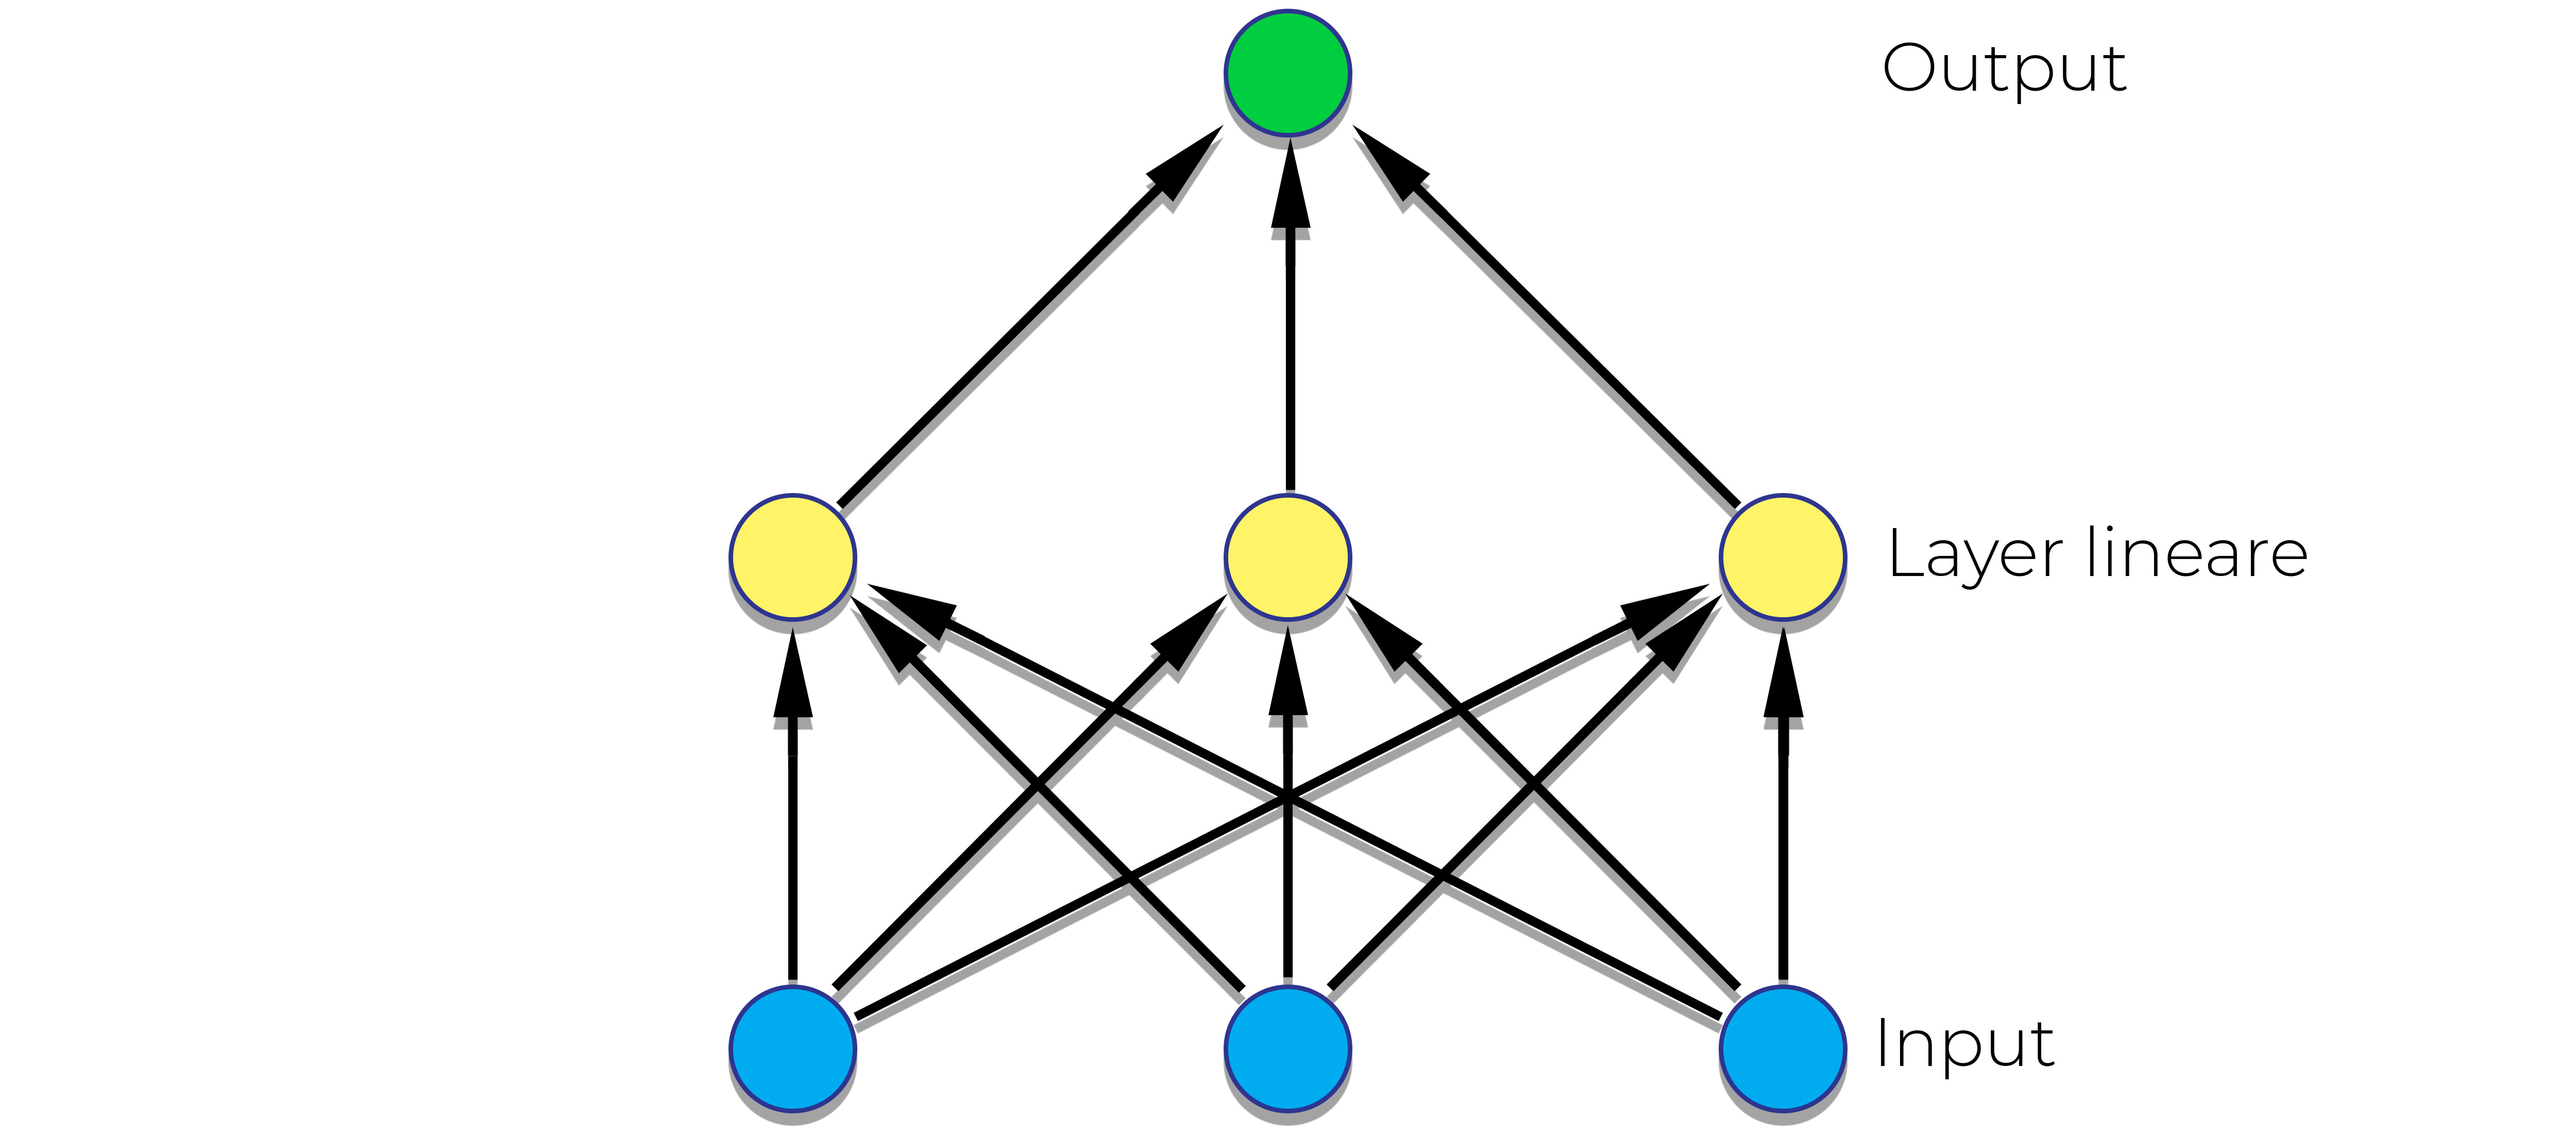
\includegraphics[width=0.8\columnwidth]{images/stateofart/double-linear-NN.jpg}
  \end{center}
  \caption{Modello a 2 strati, ancora lineare}
  \label{fig:double-linear-NN}
\end{figure}
Questo modello, però, non è ancora esente da difetti: infatti, essendo questo ancora un modello lineare, è possibile semplificarlo, ottenendo il primo grafico. È utile, allora, inserire una non-linearità all'interno del modello, che chiameremo \textit{funzione di attivazione}: ora avremo, oltre ai layer lineari, una funzione tra di loro non lineare. Grazie a essa, l'aggiunta di nuovi strati è diventata significativa: non sarebbe più possibile semplificare il sistema ad uno lineare.
\begin{figure}[H]
  \begin{center}
    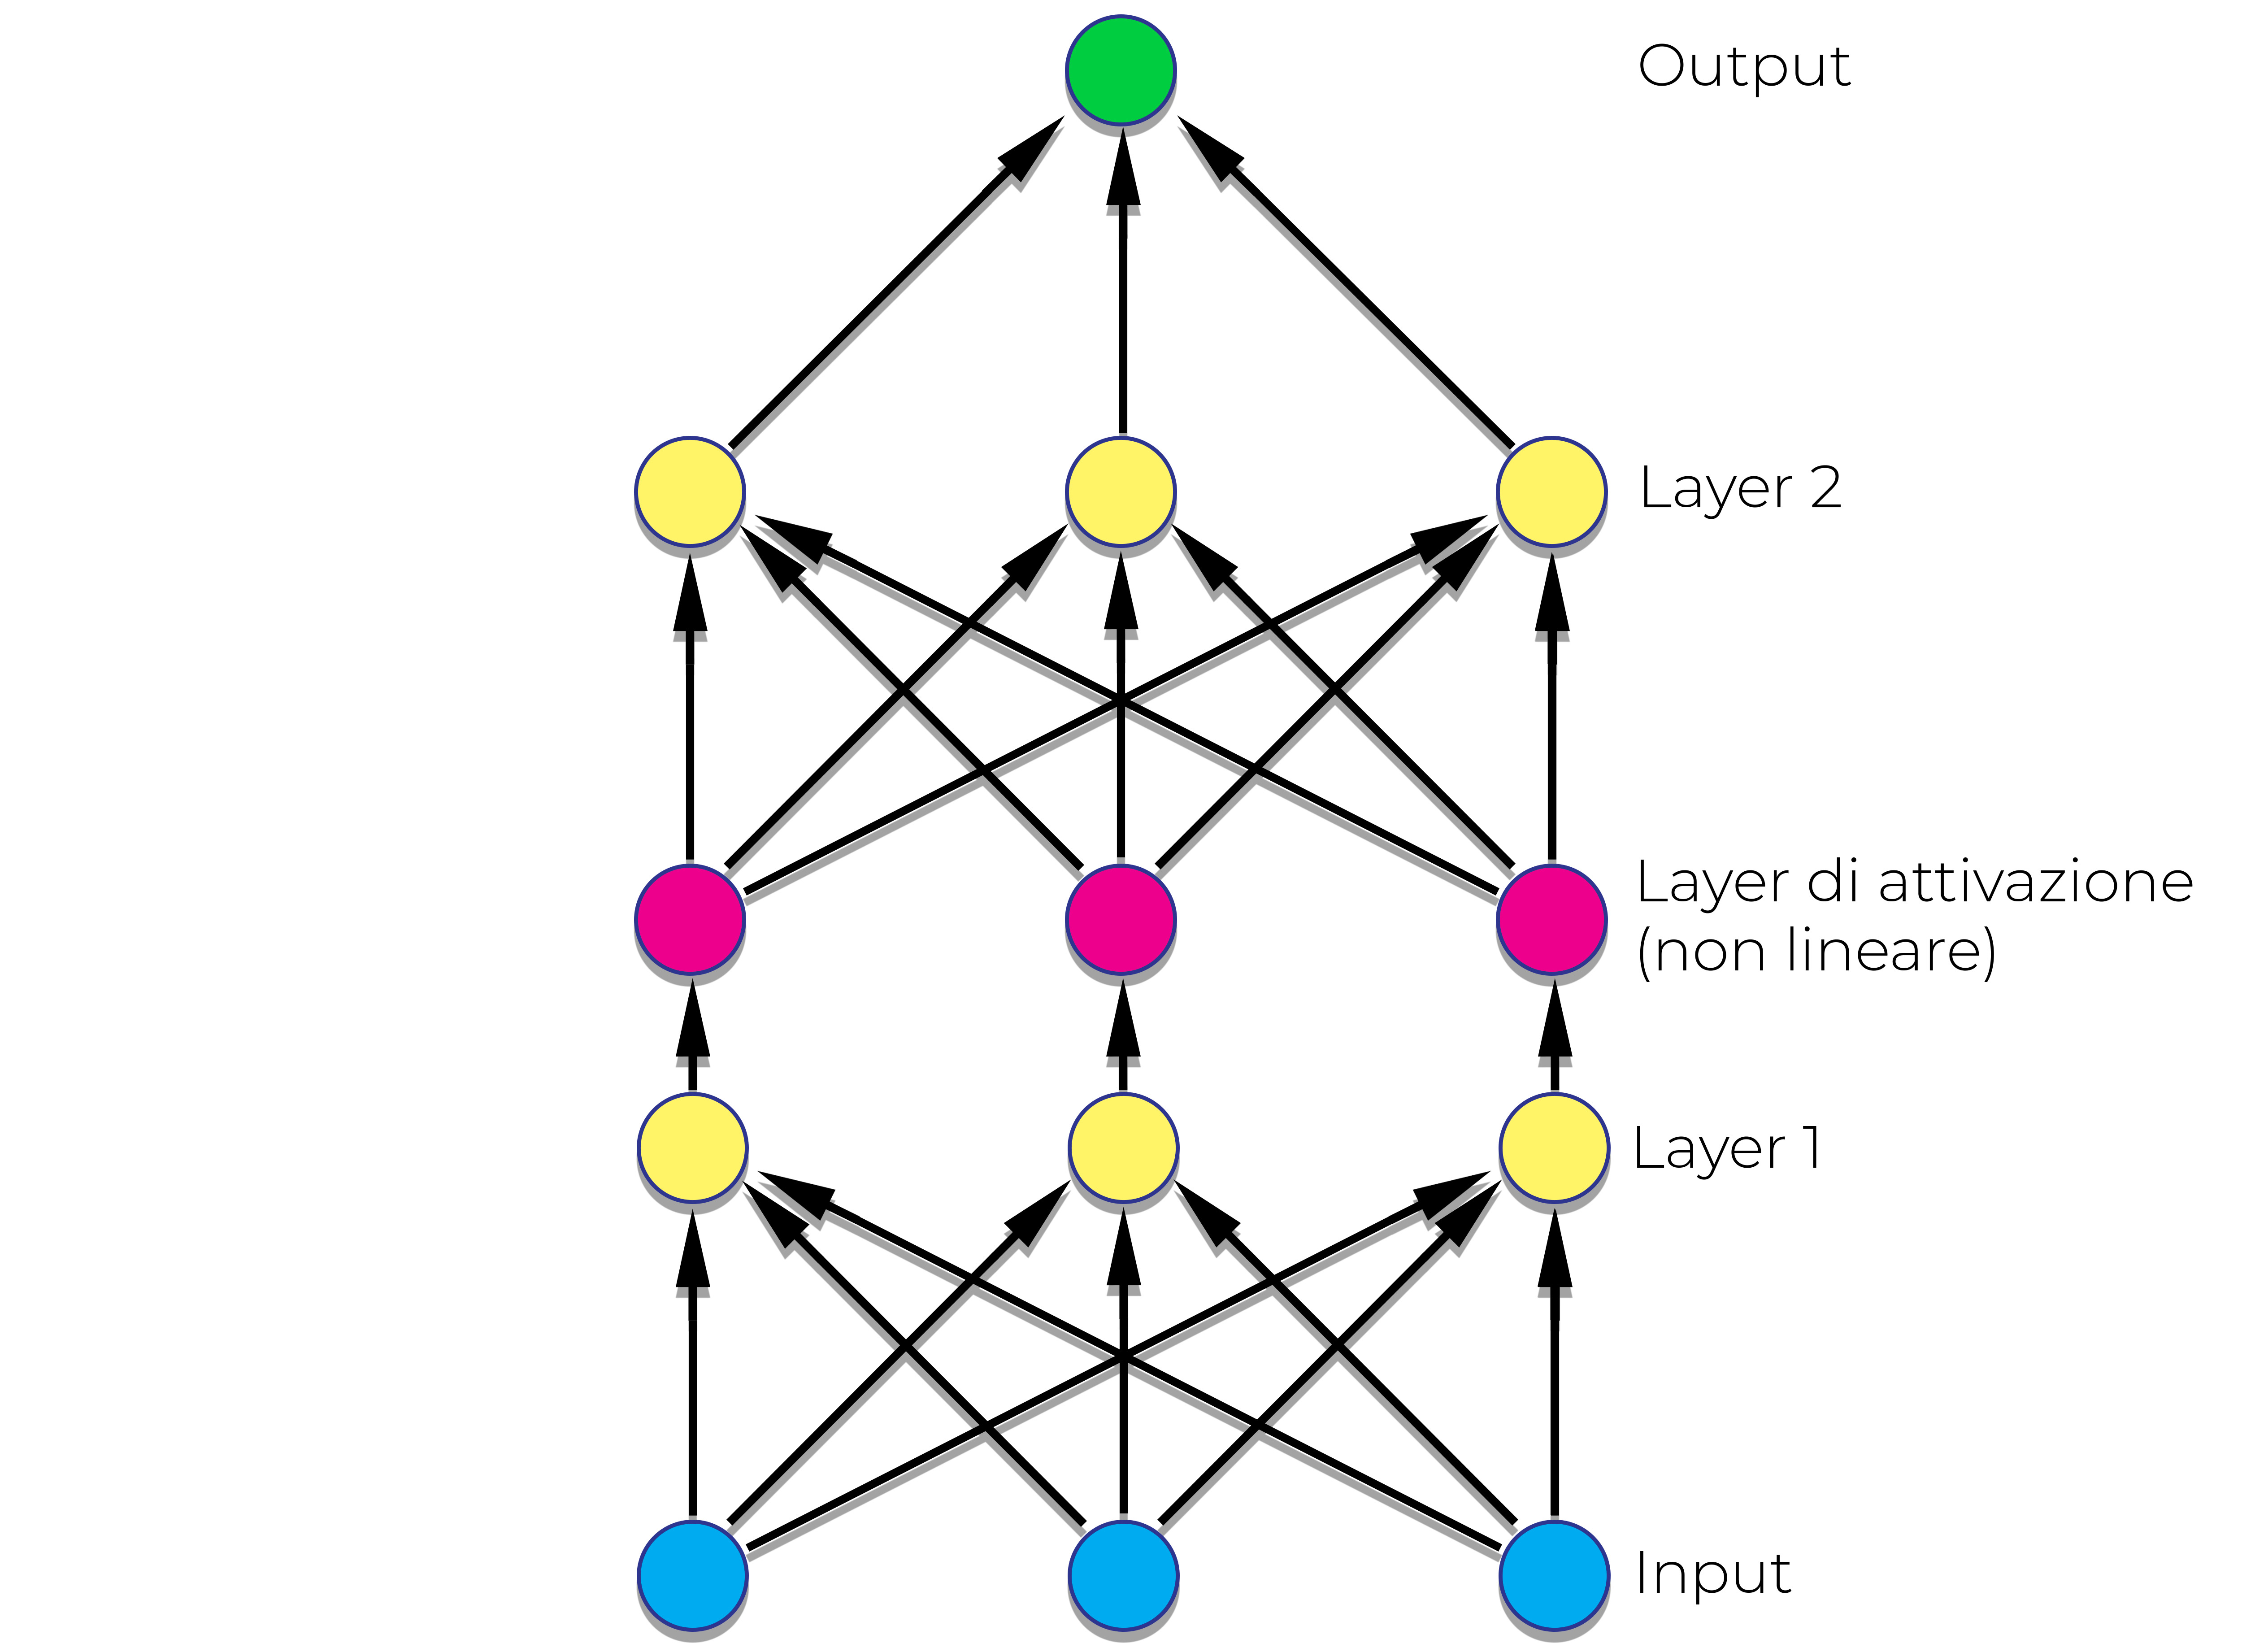
\includegraphics[width=0.8\columnwidth]{images/stateofart/real-NN.jpg}
  \end{center}
  \caption{Rete neurale}
  \label{fig:real-NN}
\end{figure}
Tra le funzioni di attivazione, citiamo la funzione sigmoidea $F(x)=\frac{1}{1+e^{-x}}$, o la \textit{Rectified Linear Unit} (ReLU) $F(x)=max(0,x)$. Non esiste una funzione di attivazione più corretta delle altre: ogni problema avrà una configurazione dei layer e delle loro attivazioni diversa. Trovare la configurazione corretta della rete neurale è la sfida più grande nel lavoro di \textit{data analysis}. \\
Avremo ora quindi un modello capace di ottenere degli output date le input features. Ma come possiamo addestrarlo per ottenere dei risultati validi? Una soluzione ricorrente è quella della \textbf{retropropagazione dell'errore}, o backpropagation. Durante questo processo, la rete neurale calcola il gradiente dell'errore (ottenuto da una funzione di \textit{loss}) sull'output, rispettivamente ai vari pesi degli strati. Questo permette alla rete neurale di individuare quali nodi hanno più effetto sulla generazione dell'errore, e di conseguenza, regolarne i pesi per ridurre l'errore. Fatto ciò sullo strato più vicino all'output, si tratta solo di ripetere il procedimento "\textit{a salire}" per ogni layer della rete neurale.
\section{Assistenti vocali}
\label{section:vocal_assistants}
Gli assistenti vocali sono software in grado di interpretare dialoghi umani e rispondere attraverso voci sintetizzate. Alcuni esempi famosi sono \textit{Apple Siri, Amazon Alexa, Google Assistant}. Gli utenti possono effettuare domande, controllare dispositivi di domotica, e svolgere un numero di operazioni in continua espansione\cite{article:introduction_to_va}. Il software rimane costantemente in attesa della pronuncia di una \textit{wake word} da parte dell'utente; una volta riconosciuta questa parola, si mette in ascolto di comandi. La richiesta viene quindi tradotta in testo tramite un motore di \textit{Speech To Text} ed interpretata dal software. Quest'ultima è senz'altro la parte più complessa: il compito di interpretazione di linguaggio naturale è reso complesso dalle svariate sfaccettature che ogni diversa lingua presenta. Interpretata la richiesta, l'assistente procede con le operazioni collegate, e prepara una risposta testuale da dare all'utente. Questa risposta verrà poi sintetizzata in audio da un motore di \textit{Text To Speech}. I moderni dispositivi di assistenza vocale come Google Home o Amazon Echo si appoggiano a server in cloud per l'interpretazione delle richieste: questo permette di ridurne notevolmente le dimensioni ed i requisiti tecnici.
Lo sviluppo, negli ultimi anni, di nuove tecniche di ML, unite ad un grande incremento delle potenze di calcolo e alla disponibilità di vastissimi \textit{dataset linguistici}, hanno permesso grandi miglioramenti nella tecnologia, ma soprattutto l'applicazione ad ambiti, fino a qualche anno fa, impensabili.
\subsection{Assistenti vocali in ambito medico}
Negli anni sono emerse alcune possibili applicazioni delle tecnologie per assistenti vocali in ambito medico. La startup \textbf{Saykara} ha creato un software che permette di analizzare le conversazioni medico-paziente, allo scopo di creare schede cliniche accurate senza dover impegnare il medico in lunghe procedure di \textit{data entry}.
Un report \cite{article:voicebot_research} di Voicebot, organizzazione per la diffusione degli assistenti vocali, afferma che il 52\% degli intervistati sarebbe intenzionato ad utilizzare assistenti vocali in ambito medico nel futuro. Solo il 7.5\% (1 su 13) l'ha già fatto.
\begin{figure}[H]
  \begin{center}
    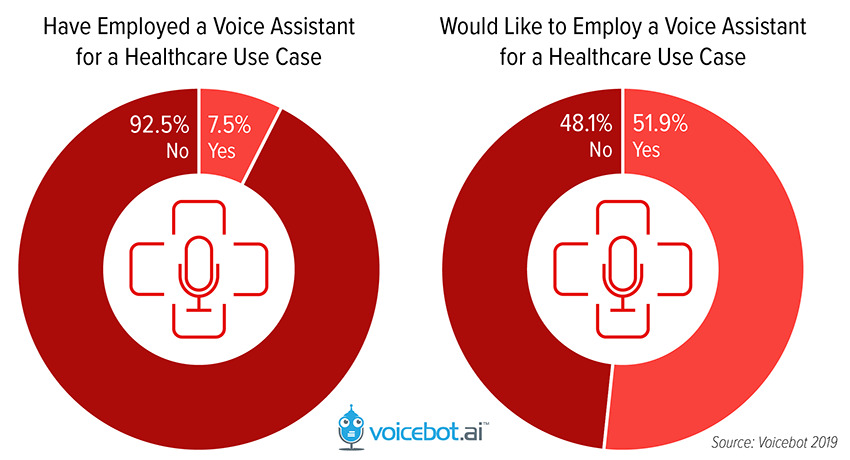
\includegraphics[width=0.8\columnwidth]{images/voice-assistant-interest-healthcare.jpg}
  \end{center}
  \caption{Percentuali di utenti che hanno utilizzato/vorrebbero utilizzare assistenti vocali in ambito medico}
  \label{fig:consumer-interest}
\end{figure}
È interessante notare come anche le fasce di età più avanzate siano, seppur con percentuali più basse, interessate a provare simili applicazioni della tecnologia.
\begin{figure}[H]
  \begin{center}
    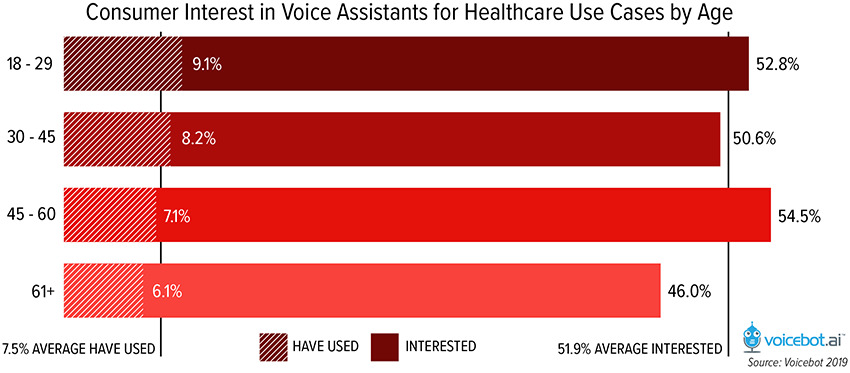
\includegraphics[width=0.8\columnwidth]{images/consumer-interest-in-voice-assistants-for-healthcare-use-cases-by-age.jpg}
  \end{center}
  \caption{Interesse dei consumatori negli assistenti vocali in ambito medico, per fasce di età}
  \label{fig:consumer-interest-forage}
\end{figure}
Un altro esempio interessante di applicazione della tecnologia in ambito medico è \textit{Dragon Medical Virtual Assistant} rilasciato da \textbf{Nuance}, una suite di strumenti vocali capaci di creare cartelle cliniche, eseguire diagnostica sul paziente, fornire risultati in diretta di ricerche mediche, supportare le operazioni di radiologia.
\newpage
\section{Triage}
\begin{wrapfigure}{r}{0.27\textwidth}
  \begin{center}
    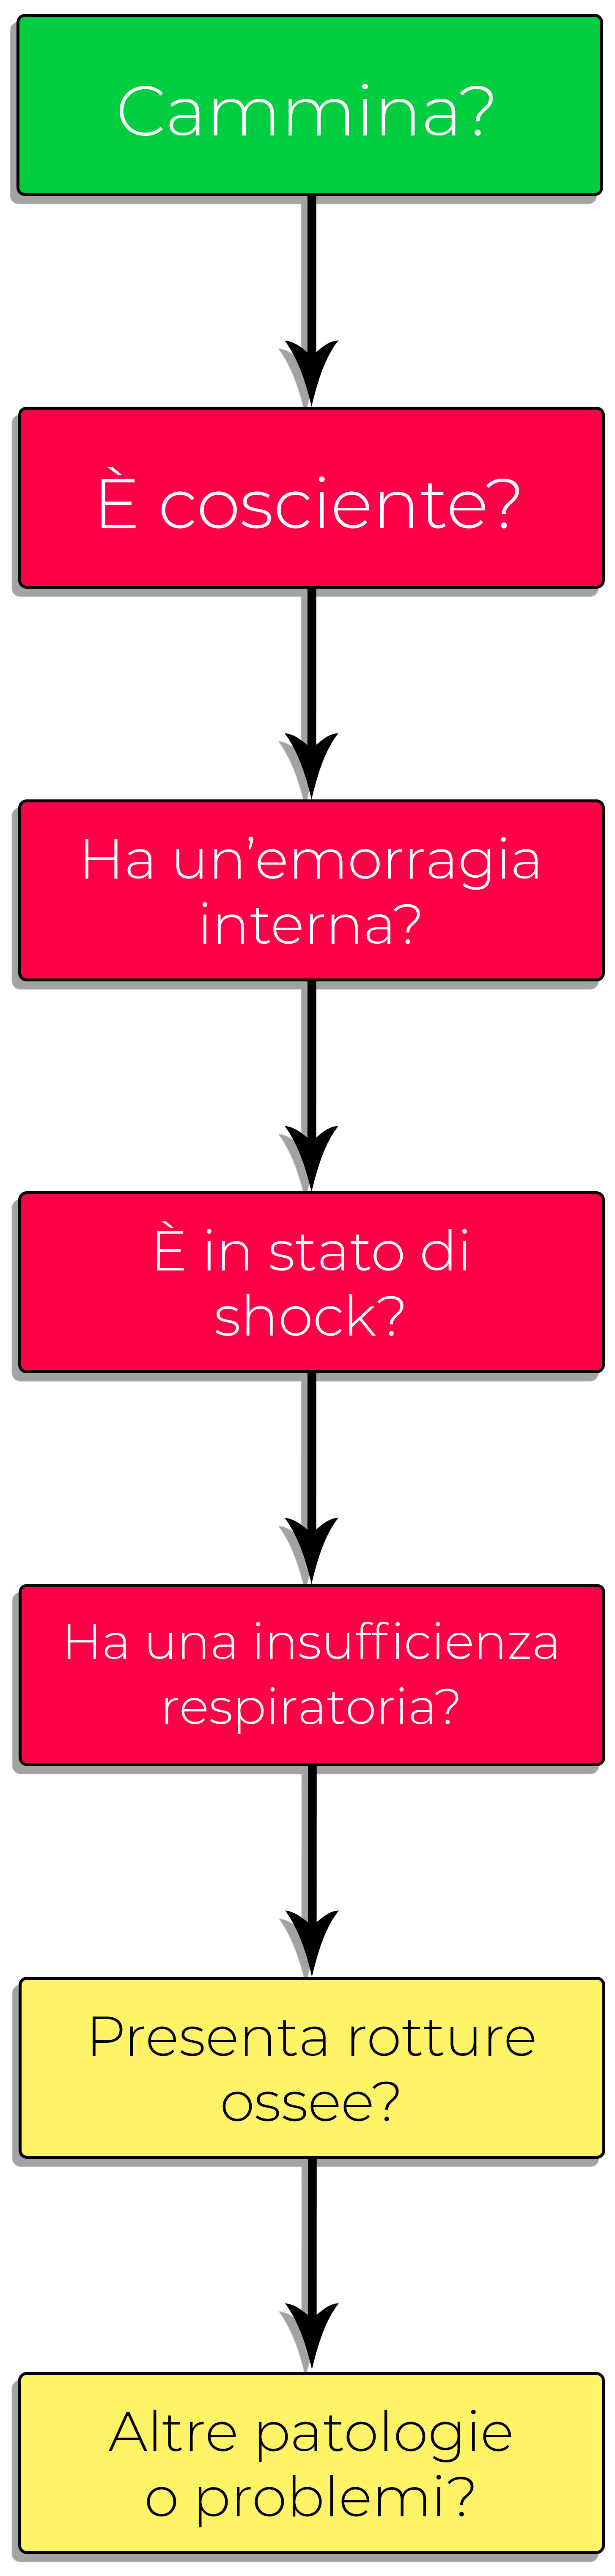
\includegraphics[width=0.25\textwidth]{images/Schema-CESIRA-ombra.jpg}
  \end{center}
  \caption{Schema del protocollo CESIRA}
\end{wrapfigure}
Il \textbf{triage} è, per definizione, il sistema utilizzato per selezionare i soggetti coinvolti in infortuni, gravi o leggeri che siano, secondo classi di emergenza, in base alla gravità delle lesioni riportate o del loro quadro clinico. Il termine nacque in ambiti di guerra (se ne cominciò a parlare durante le \textit{guerre napoleoniche}), durante i quali si classificavano i soldati feriti in base alla probabilità di sopravvivenza. Il procedimento cominciò poi, nel corso degli anni, ad essere utilizzato in ambito ospedaliero, con l'applicazione di metodi più \textit{scientifici} come il modello \textit{START}, basato su un algoritmo che prevede la verifica di sintomi visibili, frequenza respiratoria, pulsazioni, risposta ai comandi. Sebbene inizialmente le procedure di triage fossero sfruttate solo in ambito di maxiemergenze, oggi tutti i pronto soccorso italiani ne fanno uso in qualche modo. Non esiste però uno standard di codici utilizzati in ogni ospedale: le normative cambiano tra un pronto soccorso e l'altro.
Distinguiamo però, generalmente, 4 tipi di codice:
\begin{itemize}
  \item Codice \textbf{rosso}: paziente critico con cedimento di una o più funzioni vitali. \textit{Accesso immediato.}
  \item Codice \textbf{giallo}: potenziale rischio di vita o compromissione di una o più funzioni vitali. \textit{Accesso entro 15 minuti.}
  \item Codice \textbf{verde}: valutazione medica differibile nel tempo senza alcun rischio evolutivo. \textit{Accesso entro 60-90 minuti.}
  \item Codice \textbf{bianco}: paziente senza emergenza, con problematiche risolvibili a domicilio o dal medico di famiglia.
\end{itemize}
Il triage infermieristico produce quindi una \textbf{scheda di triage}, che ha valore giuridico, contenente anagrafica, data/ora di accettazione, motivo, codice colore.
Durante le emergenze è comune utilizzare il protocollo \textbf{CESIRA} (\textbf{C}oscienza, \textbf{E}morragia, \textbf{S}hock, \textbf{I}nsufficienza respiratoria, \textbf{R}otture, \textbf{A}ltro).
\subsection{Come il COVID19 ha modificato le procedure di triage}
La pandemia globale di COVID19 ha modificato i processi di triage in ospedale: lo scopo è limitare al massimo le possibilità di contagio tra i pazienti, rendendo il pronto soccorso più sicuro tanto per i pazienti, quanto per il personale sanitario. Alcuni ospedali in Inghilterra hanno addirittura iniziato a praticare triage remoto: il paziente comunica le sintomatologie online e, solo se necessario, può recarsi in ospedale per la visita medica \cite{article:digital_triage}. In Italia, ogni ospedale ha provveduto a definire delle procedure di \textbf{pre-triage} atte ad evitare il contatto tra pazienti affetti da COVID19 e non. Generalmente, si tratta di percorsi obbligati in cui i pazienti con sintomi compatibili con COVID19 (febbre, tosse, insufficienza respiratoria) vengono separati in un'\textit{area di decontaminazione} e visitati senza accedere agli ambienti del pronto soccorso comune. Nell'ospedale Maggiore di Parma sono state previste, durante i momenti di picco dell'epidemia, due tende di pre-triage esterne all'ospedale stesso.